\documentclass{article}



\usepackage{fullpage}
\usepackage{nopageno}
\usepackage{amsmath}
\usepackage{amsfonts}
\usepackage{graphicx}
\usepackage{framed}
\usepackage{xcolor}

\definecolor{dark_red}{rgb}{0.5,0.0,0.0}
\definecolor{dark_green}{rgb}{0.0,0.5,0.0}
\definecolor{dark_blue}{rgb}{0.0,0.0,0.5}

\newcommand{\dr}[1]{\textcolor{dark_red}{#1}}
\newcommand{\dg}[1]{\textcolor{dark_green}{#1}}
\newcommand{\db}[1]{\textcolor{dark_blue}{#1}}


\begin{document}


%\section{Solving Right-triangles}
%
%Given a right triangle where a single side is known, and one of the non-right angles is known (referred to henceforth as the {\bf named angle}), the process of finding the lengths of the other two sides is: 
%
%\begin{tabular}{cc}
%\parbox{0.5\textwidth}{
%\begin{itemize}
%\item If the hypotenuse \(\dr{h}\) is known, 
%	\begin{itemize}
%	\item The adjacent \(a = \dr{h\cos\theta}\)
%	\item The opposite \(o = \dr{h\sin\theta}\)
%	\end{itemize}
%\item If the adjacent \(\dg{a}\) is known, 
%	\begin{itemize}
%	\item The opposite \(o = \dg{a\tan\theta}\)
%	\item The hypotenuse \(h = \dg{a\sec\theta}\)
%	\end{itemize}
%\item If the opposite \(\db{o}\) is known, 
%	\begin{itemize}
%	\item The adjacent \(a = \db{o\cot\theta}\)
%	\item The hypotenuse \(h = \db{o\csc\theta}\)
%	\end{itemize}
%\end{itemize}
%} & \parbox{0.3\textwidth}{
%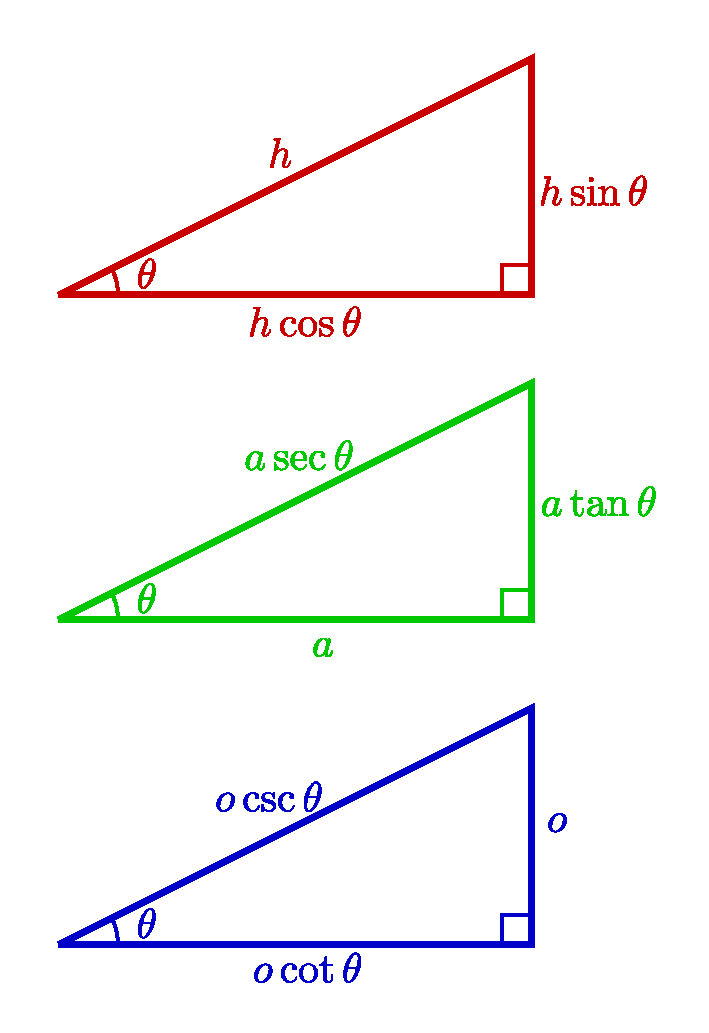
\includegraphics[width = 0.3\textwidth]{3_triangles_non_unit}
%}
%\end{tabular}
%
%
%\begin{tabular}{cc}
%\parbox{0.6\textwidth}{
%In the image to the right, \(\alpha = 35^\circ\), \(\beta = 65^\circ\), \(\gamma = 40^\circ\), \(\delta = 60^\circ\), \(\epsilon = 70^\circ\), and \(\theta = 10^\circ\). \\ ~~ \\
%\begin{itemize}
%\item \(a = 1 \cdot \cos\alpha = \cos 35^\circ \approx 0.8192\)
%\item \(b = a \cos\beta = \cos 35^\circ \cos 65^\circ \approx 0.3462\)
%\item \(c = a \sin\beta = \cos 35^\circ \sin 65^\circ \approx 0.7424\)
%\item \(d = c\tan\gamma = \cos 35^\circ \sin 65^\circ \tan 40^\circ \approx 0.6230\)
%\item \(e = c\sec\gamma = \cos 35^\circ \sin 65^\circ \sec 40^\circ \approx 0.9691\)
%\item \(f = 1 \cdot \sin\alpha = \sin 35^\circ \approx 0.5736\)
%\item \(g = f\cot\delta = \sin 35^\circ \cot 60^\circ \approx 0.3312\)
%\item \(h = f\csc\delta = \sin 35^\circ \csc 60^\circ \approx 0.6623\)
%\item \(i = 1 \cdot \cot\epsilon = \cot 70^\circ \approx 0.3640\)
%\item \(j = 1 \cdot \csc\epsilon = \csc 70^\circ \approx 1.064\)
%\item \(k = j\tan\theta = \csc 70^\circ \tan 10^\circ \approx 0.1876\)
%\item \(l = j\sec\theta = \csc 70^\circ \sec 10^\circ \approx 1.081\)
%\end{itemize}
%} & \parbox{0.4\textwidth}{
%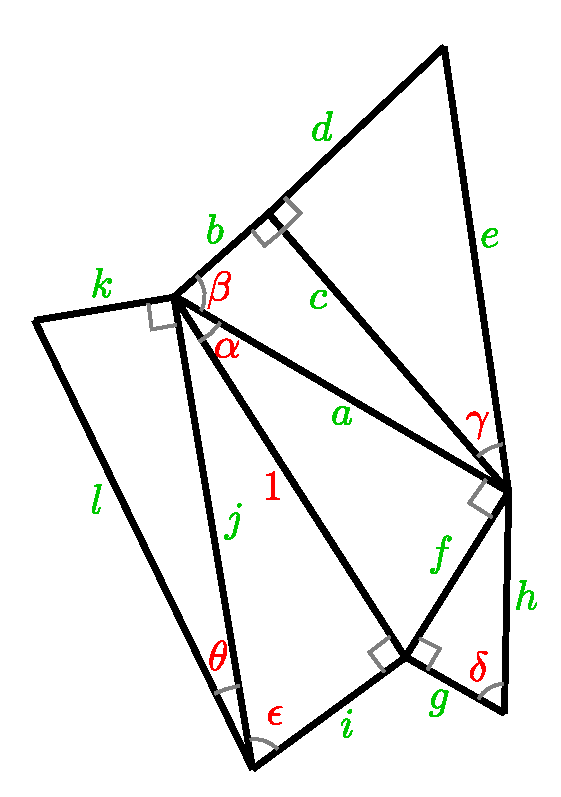
\includegraphics[width = 0.4\textwidth]{lots_of_triangles}
%}
%\end{tabular}





\section{Inverse Trigonometric Functions}

%Given a function \(f : A \rightarrow B\), whose {\bf domain} is set \(A\), and whose {\bf co-domain} is set \(B\), function \(f\) has an inverse if and only if the following holds: 
%
%\begin{itemize}
%\item There exists no two \emph{distinct} elements \(x_1\) and \(x_2\) from set \(A\) such that \(f(x_1) = f(x_2)\):
%\[\forall x_1, x_2 \in A : x_1 \neq x_2 \implies f(x_1) \neq f(x_2)\] 
%This makes \(f\) {\bf one-to-one}.
%\item For every element \(y\) from set \(B\), there exists at least one element \(x\) from set \(A\) such that \(y = f(x)\):
%\[\forall y \in B : \exists x \in A : f(x) = y\] 
%This makes \(f\) {\bf onto}.
%\end{itemize}
%
%If \(f\) is both one-to-one and onto, then for every element \(y\) from set \(B\), there exists {\bf exactly} one element \(x\) from set \(A\) such that \(y = f(x)\). This makes \(f\) a {\bf bijection}. Only bijective functions have inverses. 
%
%The inverse function \(f^{-1} : B \rightarrow A\) of function \(f\) is defined such that for every element \(y\) from set \(B\), \(f^{-1}(x)\) is the one and only element of \(A\) where \(f(f^{-1}(y)) = y\).
%\begin{itemize}
%\item For every element \(x\) from set \(A\), \(f^{-1}(f(x)) = x\):
%\[\forall x \in A : f^{-1}(f(x)) = x\]
%\item For every element \(y\) from set \(B\), \(f(f^{-1}(y)) = y\):
%\[\forall y \in B : f(f^{-1}(y)) = y\]
%\end{itemize}
%
%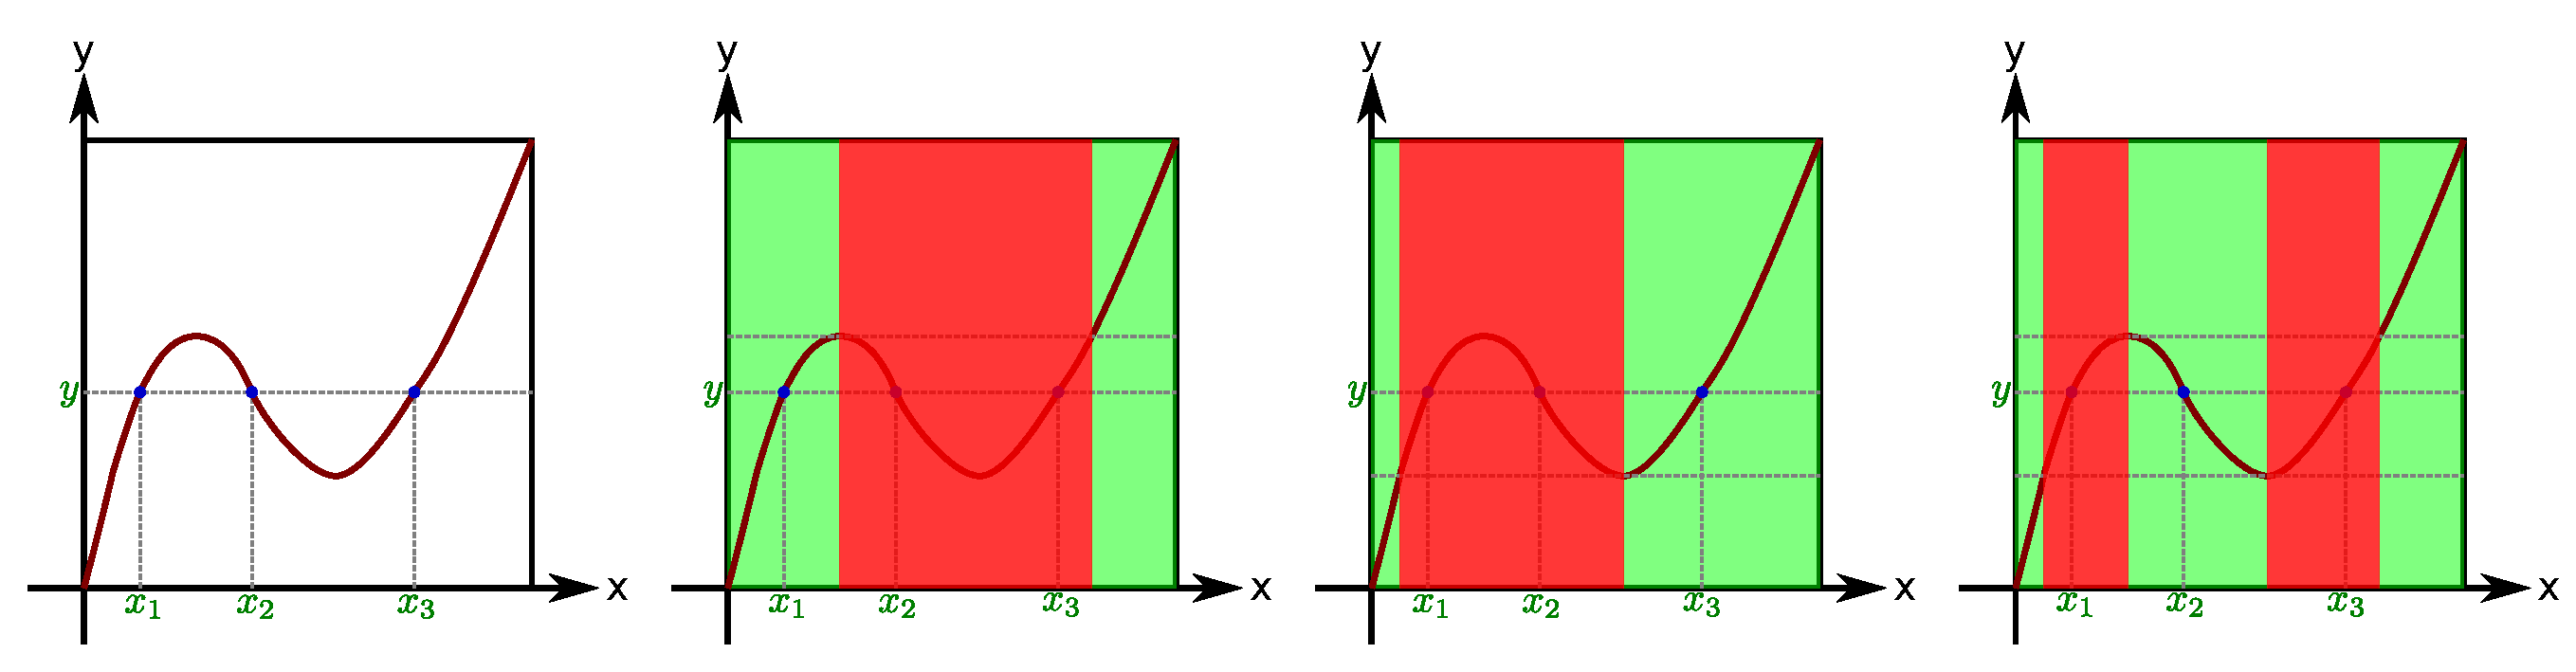
\includegraphics[scale = 0.34]{one_to_one_example_1}
%
%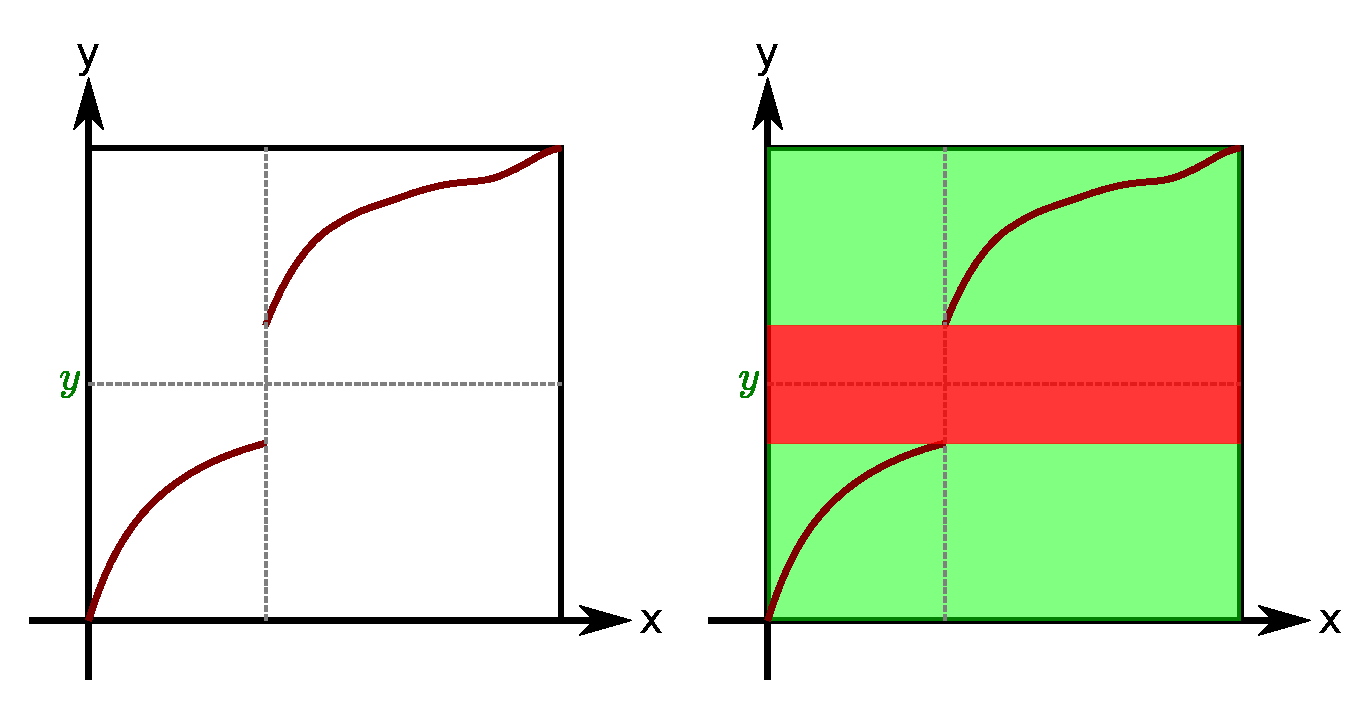
\includegraphics[scale = 0.34]{onto_example_1}
%
%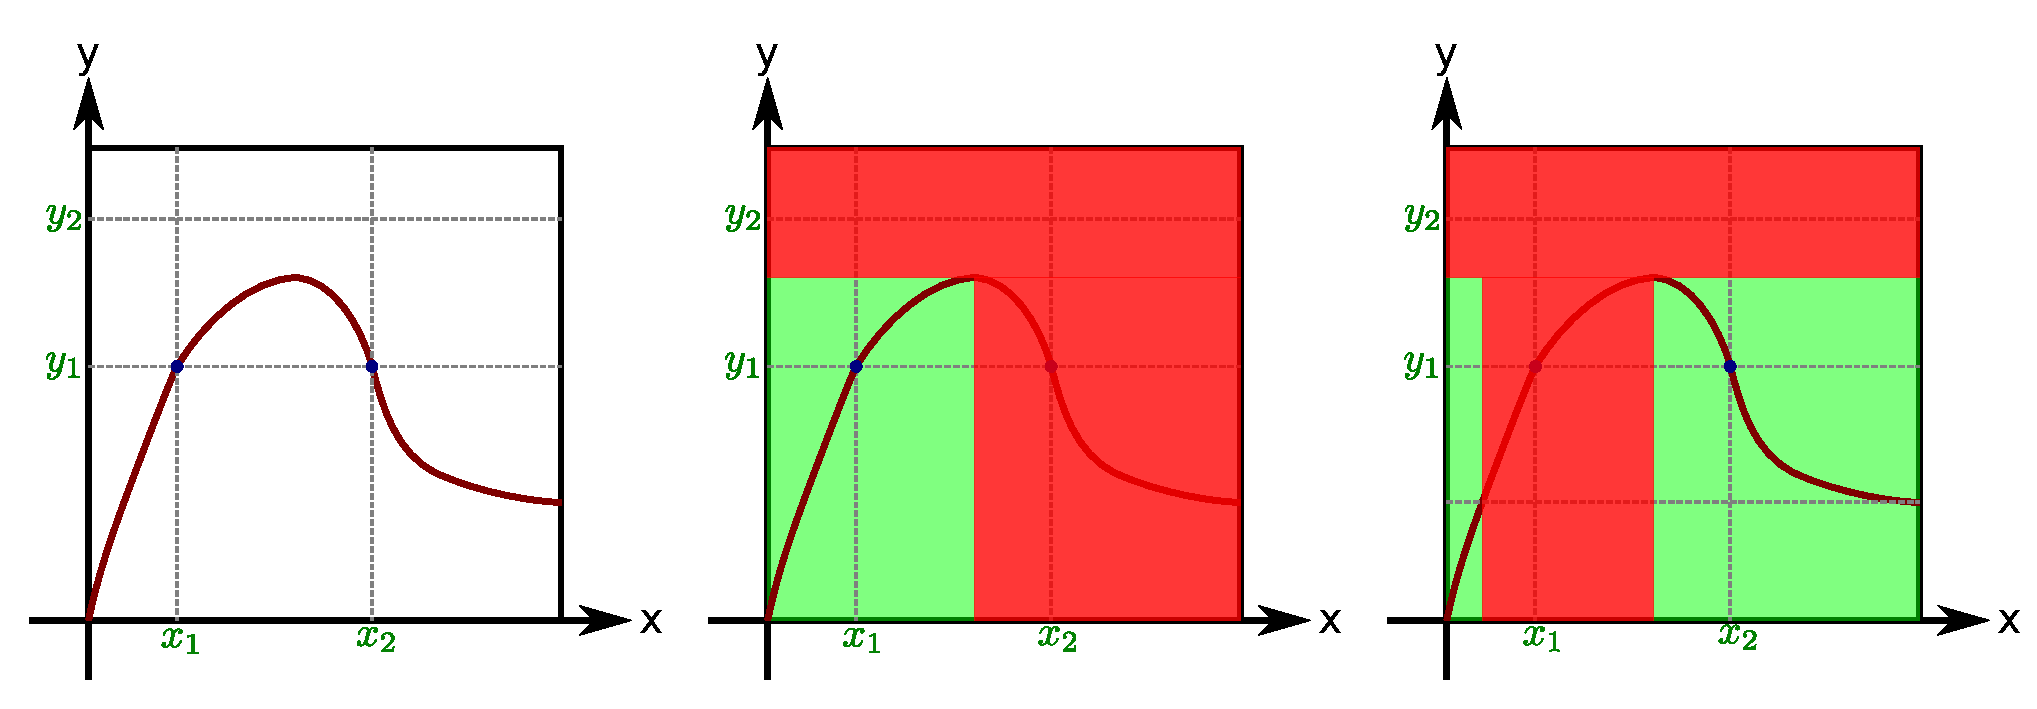
\includegraphics[scale = 0.34]{bijective_example_1}

With the trigonometric functions, the ratio between two sides is computed from the angle. In many cases the reverse is sought: to compute the angle given the side lengths. Inverses to the trigonometric functions \(\cos\), \(\sin\), and \(\tan\) will be formulated. 



\subsection{The inverse cosine: $\cos^{-1} y$}

The function \(f(\theta) = \cos\theta\) is {\bf not} one-to-one. Without modification to the domain, no inverse to the function \(f(\theta) = \cos\theta\) exists. 

The range of values attained by the function \(f(\theta) = \cos\theta\) is \([-1, 1]\), and this range is the domain of the inverse function \(f^{-1}(y) = \cos^{-1} y\).

The values of \(\cos\theta\) repeat themselves again and again as \(\theta\) changes. Hence \(\cos\theta\) is {\bf not one-to-one}. By restricting \(\theta\) to the domain \([0, \pi]\), \(\cos\theta\) changes continuously from \(1\) to \(-1\) as \(\theta\) increases from \(0\) to \(\pi\). Every value from the range \([-1,1]\) is visited exactly once, so \(\cos\theta\) is now {\bf one-to-one}.  

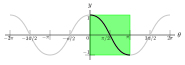
\includegraphics[width = \textwidth]{making_cos_bijective}

With the domain of \(\cos\theta\) restricted to \([0, \pi]\), the inverse function \(\cos^{-1}\) has the domain \([-1, 1]\) and the range \([0, \pi]\). The inverse is referred to as the ``inverse cosine" or the ``arc-cosine". The arc-cosine is often denoted by any of the following:

\begin{itemize}
\item \(\arccos y\)
\item \(\text{acos} y\)
\item \(\cos^{-1} y\) 
\end{itemize}

The notation of \(\cos^{-1} y\) for the inverse cosine is the reason \(\cos^{-1} y\) {\bf does not} denote \((\cos y)^{-1} = \frac{1}{\cos y}\). \(\frac{1}{\cos\theta}\) is actually \(\sec\theta\).

The inverse cosine satisfies the following properties:
\begin{itemize}
\item \(\forall \theta \in [0, \pi] : \cos^{-1}(\cos\theta) = \theta\)
\item \(\forall y \in [-1, +1] : \cos(\cos^{-1}y) = y\)
\end{itemize}



\subsection{The inverse sine: $\sin^{-1} y$}

The function \(f(\theta) = \sin\theta\) is {\bf not} one-to-one. Without modification to the domain, no inverse to the function \(f(\theta) = \sin\theta\) exists. 

The range of values attained by the function \(f(\theta) = \sin\theta\) is \([-1, 1]\), and this range is the domain of the inverse function \(f^{-1}(y) = \sin^{-1} y\).

The values of \(\sin\theta\) repeat themselves again and again as \(\theta\) changes. Hence \(\sin\theta\) is {\bf not one-to-one}. By restricting \(\theta\) to the domain \([-\pi/2, \pi/2]\), \(\sin\theta\) changes continuously from \(-1\) to \(1\) as \(\theta\) increases from \(-\pi/2\) to \(\pi/2\). Every value from the range \([-1,1]\) is visited exactly once, so \(\sin\theta\) is now {\bf one-to-one}.  

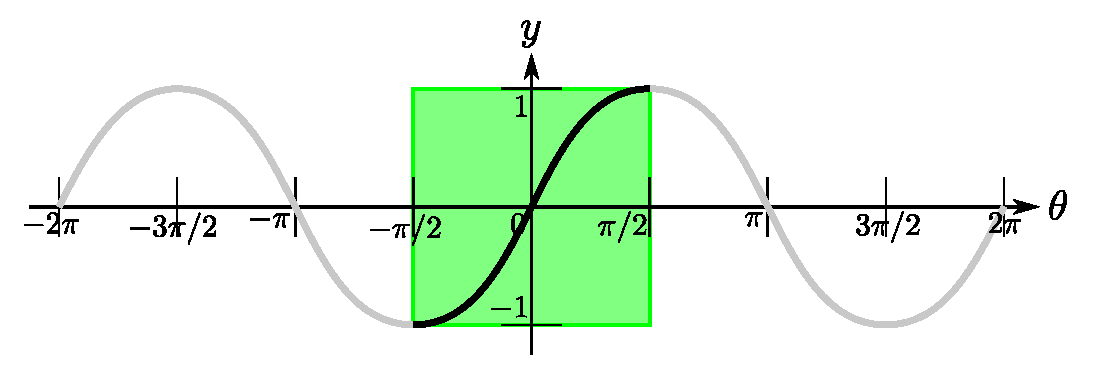
\includegraphics[width = \textwidth]{making_sin_bijective}

With the domain of \(\sin\theta\) restricted to \([-\pi/2, \pi/2]\), the inverse function \(\sin^{-1}\) has the domain \([-1, 1]\) and the range \([-\pi/2, \pi/2]\). The inverse is referred to as the ``inverse sine" or the ``arc-sine". The arc-sine is often denoted by any of the following:

\begin{itemize}
\item \(\arcsin y\)
\item \(\text{asin} y\)
\item \(\sin^{-1} y\) 
\end{itemize}

The notation of \(\sin^{-1} y\) for the inverse sine is the reason \(\sin^{-1} y\) {\bf does not} denote \((\sin y)^{-1} = \frac{1}{\sin y}\). \(\frac{1}{\sin\theta}\) is actually \(\csc\theta\).

The inverse sine satisfies the following properties:
\begin{itemize}
\item \(\forall \theta \in [-\pi/2, \pi/2] : \sin^{-1}(\sin\theta) = \theta\)
\item \(\forall y \in [-1, +1] : \sin(\sin^{-1}y) = y\)
\end{itemize}



\subsection{The inverse tangent: $\tan^{-1} y$}

The function \(f(\theta) = \tan\theta\) is {\bf not} one-to-one. Without modification to the domain, no inverse to the function \(f(\theta) = \tan\theta\) exists. 

The range of values attained by the function \(f(\theta) = \tan\theta\) is the entire set of real numbers \(\mathbb{R}\), and this range is the domain of the inverse function \(f^{-1}(y) = \tan^{-1} y\).

The values of \(\tan\theta\) repeat themselves again and again as \(\theta\) changes. Hence \(\tan\theta\) is {\bf not one-to-one}. By restricting \(\theta\) to the domain \((-\pi/2, \pi/2)\), \(\tan\theta\) changes continuously from \(-\infty\) to \(+\infty\) as \(\theta\) increases from \(-\pi/2\) to \(\pi/2\). Every real value is visited exactly once, so \(\tan\theta\) is now {\bf one-to-one}.  

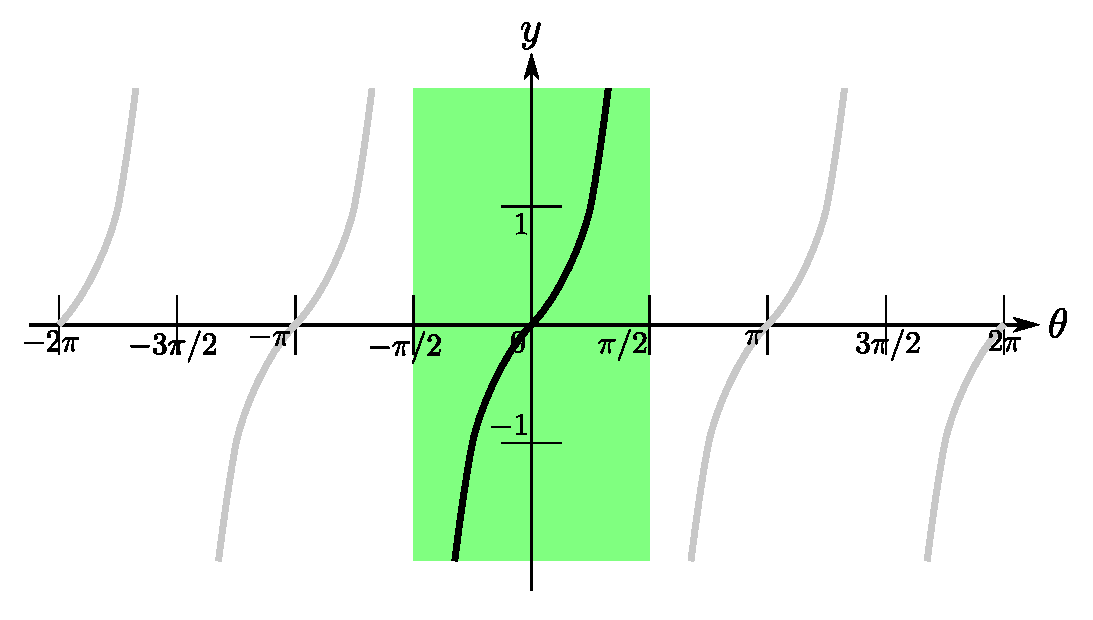
\includegraphics[width = \textwidth]{making_tan_bijective}

With the domain of \(\tan\theta\) restricted to \((-\pi/2, \pi/2)\), the inverse function \(\tan^{-1}\) has the domain \(\mathbb{R}\) (the set of real numbers) and the range \((-\pi/2, \pi/2)\). The inverse is referred to as the ``inverse tangent" or the ``arc-tan". The arc-tan is often denoted by any of the following:

\begin{itemize}
\item \(\arctan y\)
\item \(\text{atan} y\)
\item \(\tan^{-1} y\) 
\end{itemize}

The notation of \(\tan^{-1} y\) for the inverse tangent is the reason \(\tan^{-1} y\) {\bf does not} denote \((\tan y)^{-1} = \frac{1}{\tan y}\). \(\frac{1}{\tan\theta}\) is actually \(\cot\theta\).

The inverse tangent satisfies the following properties:
\begin{itemize}
\item \(\forall \theta \in (-\pi/2, \pi/2) : \tan^{-1}(\tan\theta) = \theta\)
\item \(\forall y \in \mathbb{R} : \tan(\tan^{-1}y) = y\)
\end{itemize}





\section{Using the inverse trigonometric functions}

\begin{tabular}{cc}
\parbox{0.5\textwidth}{
\begin{itemize}
\item If the adjacent \(a\) and opposite \(o\) is known, then the tangent of the named angle \(\theta\) is \(\tan\theta = o/a\). Therefore \(\theta = \tan^{-1}(o/a)\). \\ ~ \\
\item If the hypotenuse \(h\) and opposite \(o\) is known, then the sine of the named angle \(\theta\) is \(\sin\theta = o/h\). Therefore \(\theta = \sin^{-1}(o/h)\). \\ ~ \\ 
\item If the hypotenuse \(h\) and adjacent \(a\) is known, then the cosine of the named angle \(\theta\) is \(\cos\theta = a/h\). Therefore \(\theta = \cos^{-1}(a/h)\). \\ ~ \\
\end{itemize}
} & \parbox{0.3\textwidth}{
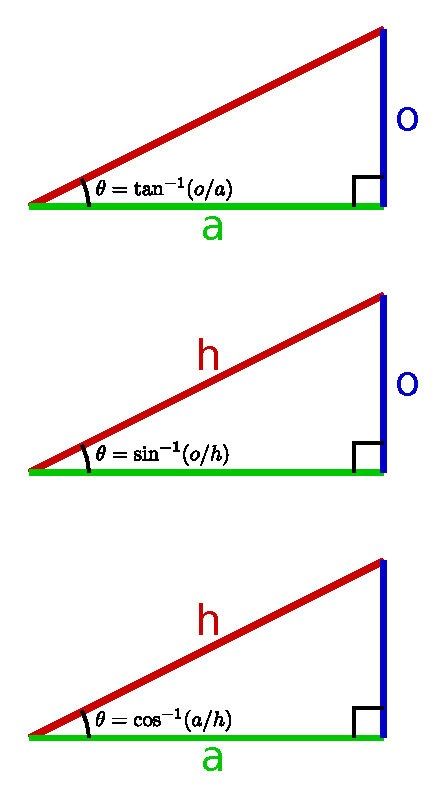
\includegraphics[width = 0.3\textwidth]{inverse_trig_scenarios}
}
\end{tabular}


\parbox{0.5\textwidth}{
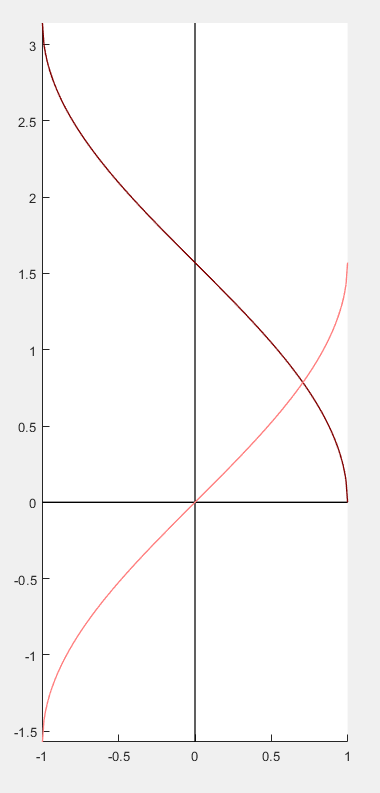
\includegraphics[scale = 0.5]{arccos_and_arcsin.png} \\
dark red \(= \arccos\theta\); ~~~ light red \(= \arcsin\theta\)
} 

\parbox{0.5\textwidth}{
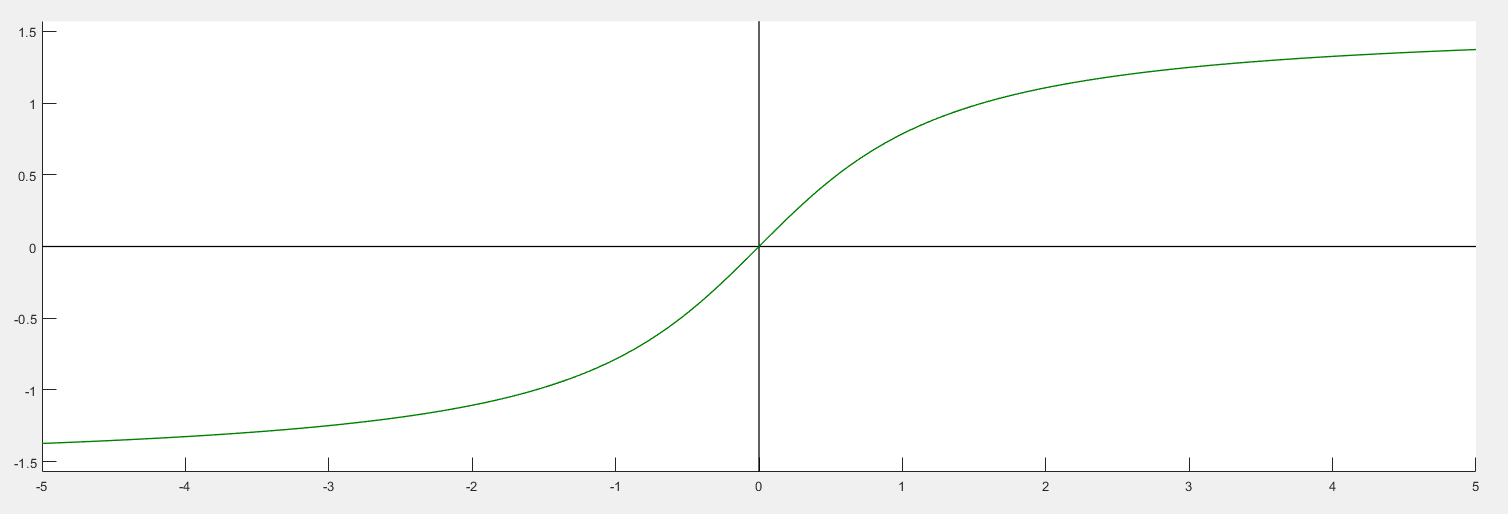
\includegraphics[scale = 0.3]{arctan.png} \\
dark green \(= \arctan\theta\)
} 

\textbf{Examples:}
\begin{itemize}
\item Given a right triangle where the adjacent is \(a = 3\) and the opposite is \(o = 4\), then the named angle is \(\theta = \tan^{-1}(o/a) \approx 53.1301^\circ\).
\item Given a right triangle where the opposite is \(o = 3.000 \times 10^3\) and the hypotenuse is \(h = 1.000 \times 10^4\), then the named angle is \(\theta = \sin^{-1}(o/h) \approx 17.4576^\circ\). 
\item Given a right triangle where the adjacent is \(a = 7.467 \times 10^{-6}\) and the hypotenuse is \(h = 2.345 \times 10^{-5}\), then the named angle is \(\theta = \cos^{-1}(a/h) \approx 71.4325^\circ\).
\end{itemize}



\subsection{The leaning plank}

\begin{tabular}{cc}
\parbox{0.5\textwidth}{
In the image on the right, a plank of known length \(L\), is propped against a ledge of known height \(y\). The angle of incline \(\theta\) of the plank is sought. The right triangle has the opposite \(y\) and hypotenuse \(L\) known, so the sine of angle \(\theta\) is \(\sin\theta = y/L\). Therefore \(\theta = \sin^{-1}(y/L)\). If \(L = 6.500\text{m}\) and \(y = 0.5000\text{m}\), then \(\theta \approx 4.41173^\circ\). 
} & \parbox{0.5\textwidth}{
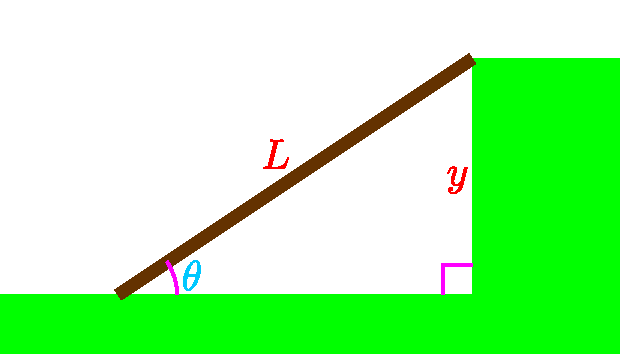
\includegraphics[width = 0.5\textwidth]{leaning_plank}
}
\end{tabular}



\subsection{The leaning plank 2}

\begin{tabular}{cc}
\parbox{0.5\textwidth}{
In the image on the right, a plank of known length \(L\), is propped against a ledge, and spans a known horizontal distance of \(x\). The angle of incline \(\theta\) of the plank is sought. The right triangle has the adjacent \(x\) and hypotenuse \(L\) known, so the cosine of angle \(\theta\) is \(\cos\theta = x/L\). Therefore \(\theta = \cos^{-1}(x/L)\). If \(L = 6.500\text{m}\) and \(x = 5.000\text{m}\), then \(\theta \approx 39.7151^\circ\). 
} & \parbox{0.5\textwidth}{
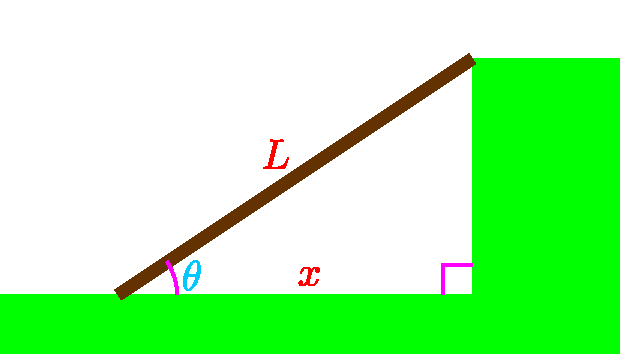
\includegraphics[width = 0.5\textwidth]{leaning_plank_2}
}
\end{tabular}



\subsection{The Sundial}

\begin{tabular}{cc}
\parbox{0.5\textwidth}{
In the image on the right, the setting is a location at the equator during one of the two equinoxes. The left of the image is the westward side. The right of the image is the eastward side. The image depicts a stick of known length \(y\) planted vertically into the ground. The stick casts a shadow of measured length \(d\). Moreover, the shadow is on the westward side. The angle \(\phi\) that the sunlight makes with the vertical direction is sought. The right triangle has the opposite \(d\) and adjacent \(y\) known, so the tangent of angle \(\phi\) is \(\tan\phi = d/y\). Therefore \(\phi = \tan^{-1}(d/y)\). The angle \(\phi\) can also be used to compute the time of day. The shadow is being cast on the western side, so the sun is in the east, so the time is am. If \(\phi\) is being measured in degrees, then the number of hours away from noon is \(H = \frac{12\text{hr}}{180^\circ}\phi\). The time would be \(T = 12\text{hr} - H\)
} & \parbox{0.5\textwidth}{
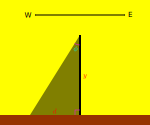
\includegraphics[width = 0.5\textwidth]{sundial}
}
\end{tabular}

For example, fixing \(y\) at \(10\text{m}\), then if:
\begin{itemize}
\item \(d = 20\text{m}\), then \(\phi \approx 63.4349^\circ\), so \(H = 4.22899\text{hr}\), so \(T = 7.77101\text{hr} = 7\text{hr} + 46\text{min} = 7\!\!:\!\!46\text{am}\). 
\item \(d = 15\text{m}\), then \(\phi \approx 56.3099^\circ\), so \(H = 3.75399\text{hr}\), so \(T = 8.24601\text{hr} = 8\text{hr} + 15\text{min} = 8\!\!:\!\!15\text{am}\). 
\item \(d = 10\text{m}\), then \(\phi = 45^\circ\), so \(H = 3\text{hr}\), so \(T = 9\text{hr} = 9\!\!:\!\!00\text{am}\). 
\item \(d = 5\text{m}\), then \(\phi \approx 26.5651^\circ\), so \(H = 1.77101\text{hr}\), so \(T = 10.2290\text{hr} = 10\text{hr} + 14\text{min} = 10\!\!:\!\!14\text{am}\).
\item \(d = 1\text{m}\), then \(\phi \approx 5.71059^\circ\), so \(H = 0.380706\text{hr}\), so \(T = 11.6193\text{hr} = 11\text{hr} + 37\text{min} = 11\!\!:\!\!37\text{am}\).
\item \(d = 0\text{m}\), then \(\phi = 0^\circ\), so \(H = 0\text{hr}\), so \(T = 12\text{hr} = 12\!\!:\!\!00\text{pm}\).
\end{itemize}




\subsection{Radius of planets}

\begin{tabular}{cc}
\parbox{0.5\textwidth}{
In the image on the right, a planet with an {\bf unknown} radius \(R\) is shown. A tower of {\bf known} height \(h\) becomes fully hidden by the curve of the planet's surface when viewed from ground level a {\bf known} distance of \(d\) from the tower's summit. With \(h\) and \(d\) known, the aim is to compute the planet's radius \(R\). The line of observation makes a right angle with the planet's radius resulting in the right triangle in the image. The Pythagorean theorem yields:
\begin{align*}
& (R + h)^2 = R^2 + d^2 \\
\iff & R^2 + 2Rh + h^2 = R^2 + d^2 \\
\iff & 2hR + h^2 = d^2 
\iff 2hR = d^2 - h^2 \\
\iff & R = \frac{d^2 - h^2}{2h} = \frac{d^2}{2h} - \frac{1}{2}h
\end{align*}
} & \parbox{0.5\textwidth}{
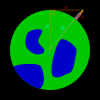
\includegraphics[width = 0.5\textwidth]{radius_of_a_planet}
}
\end{tabular}
\begin{itemize}
\item If the summit of the tower is \(d = 13\text{km}\) from the observation point, and the height that is being concealed by the planet's bulk is \(h = 100\text{m}\), then the planet's radius is 
\[R = \frac{d^2}{2h} - \frac{1}{2}h = \frac{(13\text{km})^2}{2(0.1\text{km})} - \frac{1}{2}(0.1\text{km}) \approx 844.950\text{km}\]
\item If the summit of the tower is \(d = 13\text{km}\) from the observation point, and the height that is being concealed by the planet's bulk is \(h = 10\text{m}\), then the planet's radius is 
\[R = \frac{d^2}{2h} - \frac{1}{2}h = \frac{(13\text{km})^2}{2(0.01\text{km})} - \frac{1}{2}(0.01\text{km}) \approx 8450.00\text{km}\]
\end{itemize}




\subsection{Distance between two points on the Earth's surface}

Consider two points on the Earth's surface. 
\begin{itemize}
\item Point 1: Latitude \( = 0^\circ\), Longitude \(= \theta_1\) East
\item Point 2: Latitude \( = \beta\) North, Longitude \(= \theta_2\) East (assume that \(\theta_2 > \theta_1\))
\end{itemize}

\(\theta_1\), \(\theta_2\), and \(\beta\) are all known quantities. The distance between the two points along the Earth's surface is sought. The distance between the two points along the Earth's surface is the ``great circle distance". The great circle distance is the arc length along a ``great circle" that passes through the two points. A great circle is a circle whose center is the Earth's center. For example, all longitudinal lines are great circles, while the only latitude line that is a great circle is the equator. All latitude circles save for the equator have their centers on the rotational axis, but not at the Earth's center. The image below shows the setup that enables the calculation of the great circle distance between the two points. \(\alpha = \theta_2 - \theta_1\) is the difference in longitude between the two points. The black dot is the Earth's center, and \(R_E\) is the Earth's radius. The red dot is point 1, and the green dot is point 2.

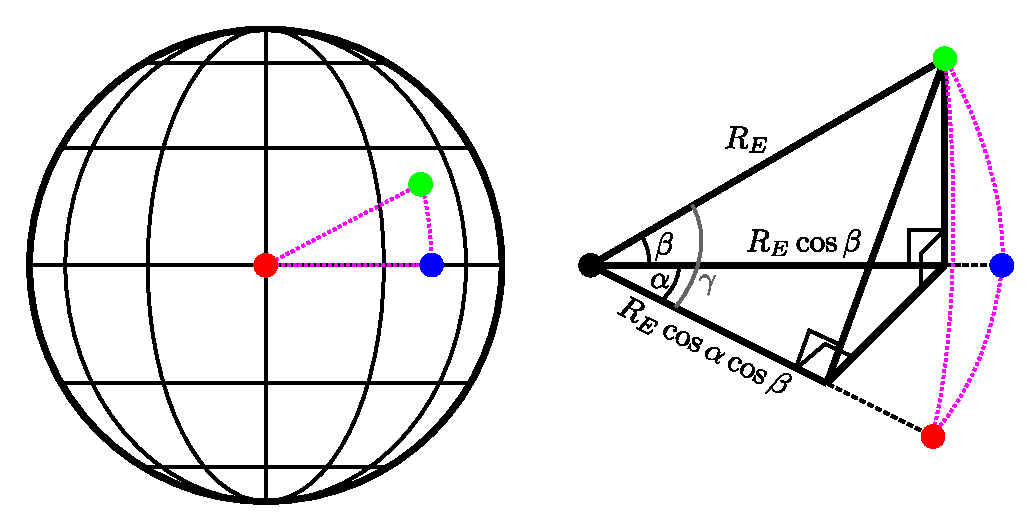
\includegraphics[width = \textwidth]{distances_with_latitude_and_longitude}

The hypotenuse of the right triangle with the named angle of \(\beta\) is \(R_E\), and using the cosine, the adjacent is \(R_E \cos\beta\). The hypotenuse of the right triangle with the named angle of \(\alpha\) is \(R_E \cos\beta\), and using the cosine, the adjacent is \(R_E \cos\alpha \cos\beta\). Lastly, with regards to the triangle with the named angle of \(\gamma\), the adjacent is \(R_E \cos\alpha \cos\beta\) and the hypotenuse is simply \(R_E\). Therefore the cosine of \(\gamma\) can be computed:
\[\cos\gamma = \frac{R_E \cos\alpha \cos\beta}{R_E} = \cos\alpha \cos\beta\]
Therefore: \(\gamma = \cos^{-1}(\cos\alpha \cos\beta)\)

\(\gamma = \cos^{-1}(\cos\alpha \cos\beta)\) is the angle corresponding to the great circle arc that connects the two points. Converting \(\gamma\) to {\bf radians}, the distance between the two points is simply \(D = R_E \gamma\).

If \(\theta_1 = 95^\circ\), \(\theta_2 = 165^\circ\), and \(\beta = 25^\circ\), then \(\alpha = \theta_2 - \theta_1 = 70^\circ\) and \(\gamma = \cos^{-1}(\cos\alpha \cos\beta) \approx 71.9422^\circ \approx 1.25563 \;\text{rad}\). Using \(R_E = 6.3781 \times 10^6\text{m}\) as the radius of the Earth, the distance between the two points is therefore \(D = R_E \gamma \approx 8.00853 \times 10^6 \text{m} = 8008.53\text{km}\)

\vspace{5mm}

\textbf{Points at equal latitude}

Now consider the two points: 
\begin{itemize}
\item Point 1: Latitude \( = \beta\) North, Longitude \(= \theta_1\) East
\item Point 2: Latitude \( = \beta\) North, Longitude \(= \theta_2\) East (assume that \(\theta_2 > \theta_1\))
\end{itemize}

\(\theta_1\), \(\theta_2\), and \(\beta\) are all known quantities. The image below shows the setup that enables the calculation of the great circle distance between the two points. \(\alpha = \theta_2 - \theta_1\) is the difference in longitude between the two points. The black dot is the Earth's center, and \(R_E\) is the Earth's radius. The red dot is point 1, and the green dot is point 2.

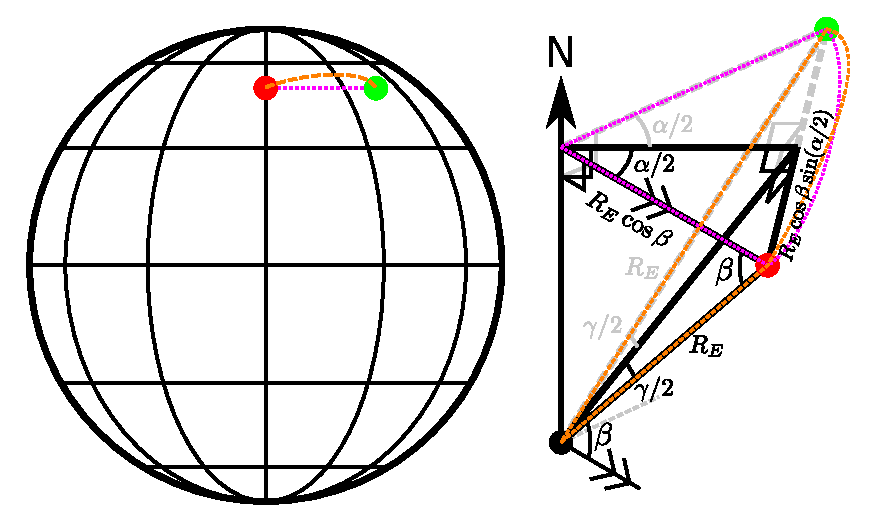
\includegraphics[width = \textwidth]{distances_at_equal_latitude}

The hypotenuse of the right triangle with the named angle of \(\beta\) is \(R_E\), and using the cosine, the adjacent is \(R_E \cos\beta\). The hypotenuse of the right triangle with the named angle of \(\alpha/2\) is \(R_E \cos\beta\), and using the sine, the opposite is \(R_E \cos\beta \sin(\alpha/2)\). Lastly, with regards to the triangle with the named angle of \(\gamma/2\), the opposite is \(R_E \cos\beta \sin(\alpha/2)\) and the hypotenuse is simply \(R_E\). Therefore the sine of \(\gamma/2\) can be computed:
\[\sin(\gamma/2) = \frac{R_E \cos\beta \sin(\alpha/2)}{R_E} = \cos\beta \sin(\alpha/2)\]
Therefore: \(\gamma/2 = \sin^{-1}(\cos\beta \sin(\alpha/2))\) which gives \(\gamma = 2\sin^{-1}(\cos\beta \sin(\alpha/2))\)

\(\gamma = 2\sin^{-1}(\cos\beta \sin(\alpha/2))\) is the angle corresponding to the great circle arc that connects the two points. Converting \(\gamma\) to {\bf radians}, the distance between the two points is simply \(D = R_E \gamma\).

If \(\theta_1 = 91^\circ\), \(\theta_2 = 135^\circ\), and \(\beta = 73^\circ\), then \(\alpha = \theta_2 - \theta_1 = 44^\circ\) and \(\gamma = 2\sin^{-1}(\cos\beta \sin(\alpha/2)) \approx 12.5758^\circ \approx 0.219489\;\text{rad}\). Using \(R_E = 6.3781 \times 10^6\text{m}\) as the radius of the Earth, the distance between the two points is therefore \(D = R_E \gamma \approx 1.39992 \times 10^6\text{m} = 1399.92\text{km}\)

To serve as contrast, the radius of the latitude circle is \(R_E\cos\beta\), and after converting \(\alpha\) to radians, the distance along the latitude circle is \((R_E\cos\beta)\alpha\). In this example, this distance is \(1.43205 \times 10^6\text{m} = 1432.05\text{km}\) which is longer than the great circle distance.



\section{Periodic Functions}

%If a function \(f(x)\) has a period of \(T\), then for every possible \(x_0 \in \mathbb{R}\):
%\[\cdots = f(x_0 - 3T) = f(x_0 - 2T) = f(x_0 - T) = f(x_0) = f(x_0 + T) = f(x_0 + 2T) = f(x_0 + 3T) = \cdots\]

%If \(m, c \in \mathbb{R}\) are arbitrary constants where \(m \neq 0\), then the function \(f(mx + c)\) over variable \(x\) has a period of \(\frac{T}{|m|}\).

A periodic function \(f(x)\) is a function that repeats the same pattern as \(x\) increases. The period \(T\) is the minimum change in \(x\) that results in a full cycle. Given a periodic function \(f(x)\) with a period of \(T\), then for all \(x \in \mathbb{R}\), 
\[\cdots = f(x - 3T) = f(x - 2T) = f(x - T) = f(x) = f(x + T) = f(x + 2T) = f(x + 3T) = \cdots\]

An example periodic function is depicted below. A full cycle is highlighted in each graph. Note that any interval of width \(T\) contains a full cycle.

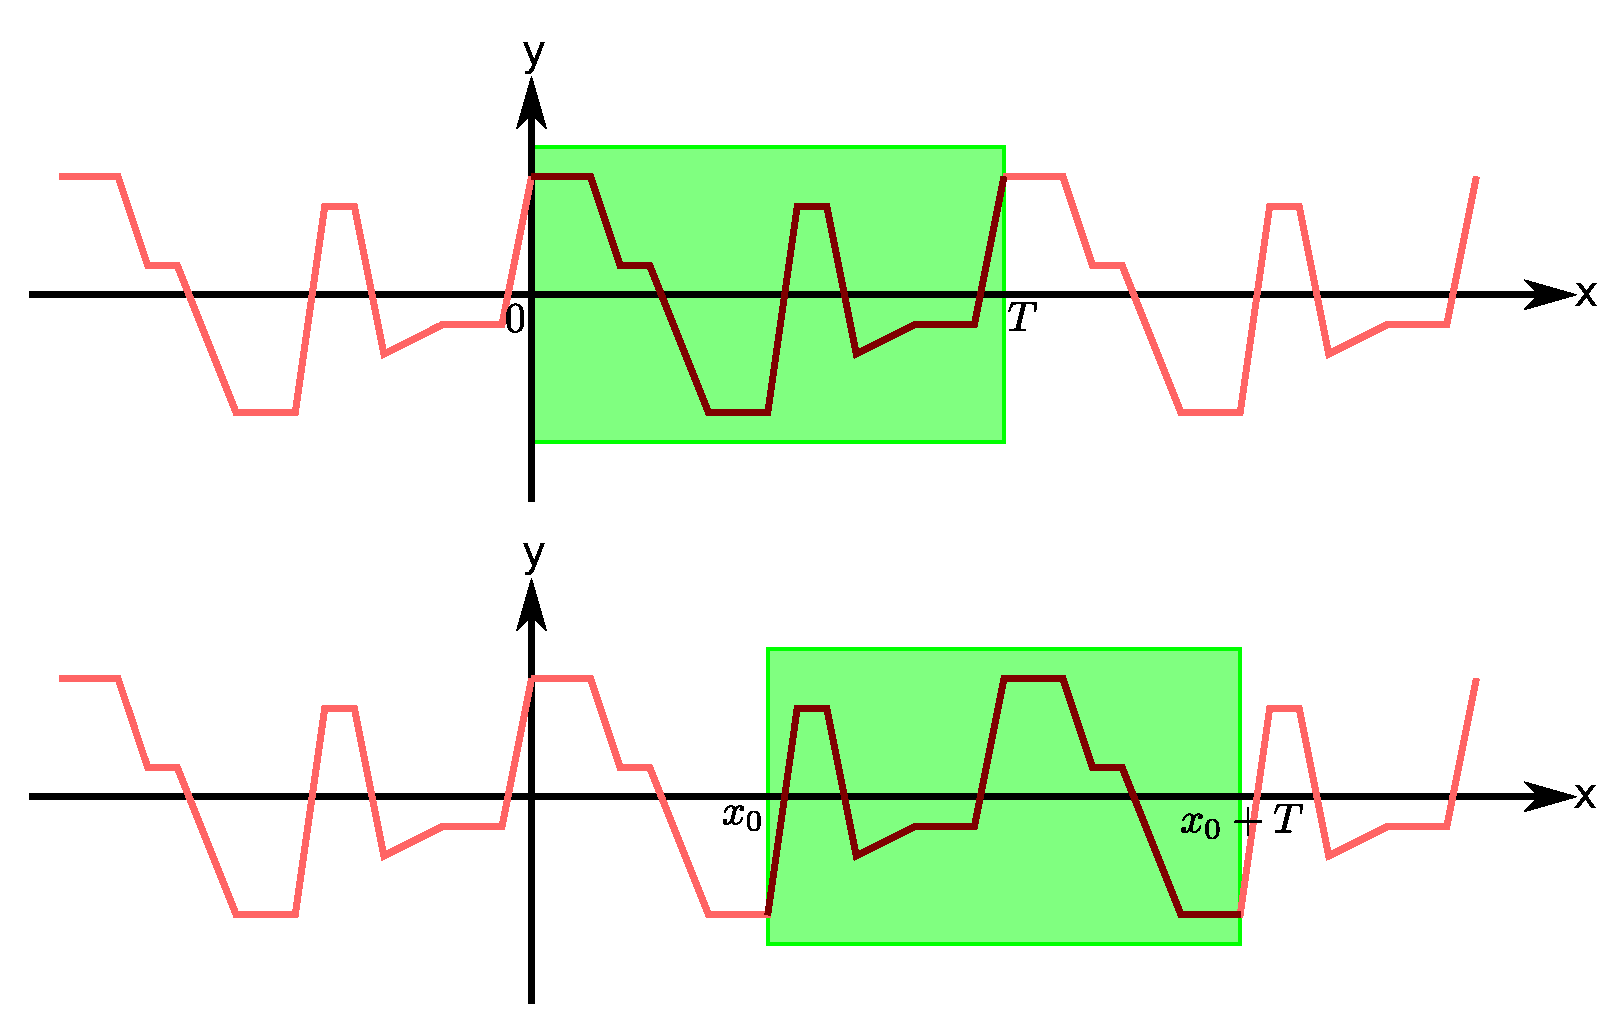
\includegraphics[width = \textwidth]{periodic_function_example_1}

\begin{itemize}
\item If \(m\) and \(c\) are arbitrary real numbers, and \(m \neq 0\), then the period of the function \(g(x) = f(mx + c)\) is \(\frac{T}{|m|}\). 
\item For the periodic function \(f(x)\), \(x\) has to increase or decrease by the amount \(T\) for \(f(x)\) to repeat itself. 
\item In the case of \(g(x) = f(mx + c)\), the expression \(mx + c\) has to increase or decrease by the amount \(T\) for \(g(x)\) to repeat itself. 
	\begin{itemize}
	\item[*] For \(mx + c\) to increase or decrease by the amount \(T\), \(mx\) has to increase or decrease by the amount \(T\) as \(c\) does not change. 
	\item[*] For \(mx\) to increase or decrease by the amount \(T\), \(x\) has to increase or decrease by the amount \(\left|\frac{T}{m}\right| = \frac{T}{|m|}\). 
	\item[*] The increase of \(\frac{T}{|m|}\) is the period of \(g(x)\).
	\end{itemize}
\end{itemize}

\begin{itemize}
\item \(\cos\theta\) has a period of \(2\pi = 360^\circ\)
\item \(\sin\theta\) has a period of \(2\pi = 360^\circ\)
\item \(\tan\theta\) has a period of \(\pi = 180^\circ\)
\item \(\sec\theta\) has a period of \(2\pi = 360^\circ\)
\item \(\cot\theta\) has a period of \(\pi = 180^\circ\)
\item \(\csc\theta\) has a period of \(2\pi = 360^\circ\)
\end{itemize}


\textbf{Examples:}
\begin{itemize}
\item  Let \(g(x) = \sin(3x + 5)\). Note that since the constant \(5\) lacks the degree \(^\circ\) symbol, \(5\) denotes a number of radians instead of degrees. Firstly, \(f(x) = \sin(x)\) has a period of \(2\pi\). For \(g(x)\) to repeat itself, \(3x + 5\) must change by \(2\pi\), so \(x\) must change by \(\frac{2\pi}{|3|} = 120^\circ\). The period of \(g(x)\) is \(\frac{2\pi}{3} = 120^\circ\).
%%%%%%%%%%%%%%%%%%%%%%%%%%%%%%%%
\item  Let \(g(x) = \cos(7 - x)\). Firstly, \(f(x) = \cos(x)\) has a period of \(2\pi\). For \(g(x)\) to repeat itself, \(7 - x\) must change by \(2\pi\), so \(x\) must change by \(\frac{2\pi}{|-1|} = 2\pi\). The period of \(g(x)\) is \(2\pi = 360^\circ\)
%%%%%%%%%%%%%%%%%%%%%%%%%%%%%%%%
\item  Let \(g(x) = \cos(2 + 4x)\). Firstly, \(f(x) = \cos(x)\) has a period of \(2\pi\). For \(g(x)\) to repeat itself, \(2 + 4x\) must change by \(2\pi\), so \(x\) must change by \(\frac{2\pi}{|4|} = \frac{\pi}{2}\). The period of \(g(x)\) is \(\frac{\pi}{2} = 90^\circ\)
%%%%%%%%%%%%%%%%%%%%%%%%%%%%%%%%
\item  Let \(g(x) = \sin(-6x)\). Firstly, \(f(x) = \sin(x)\) has a period of \(2\pi\). For \(g(x)\) to repeat itself, \(-6x\) must change by \(2\pi\), so \(x\) must change by \(\frac{2\pi}{|-6|} = \frac{\pi}{3}\). The period of \(g(x)\) is \(\frac{\pi}{3} = 60^\circ\)
%%%%%%%%%%%%%%%%%%%%%%%%%%%%%%%%
\item  Let \(g(x) = \tan(7 + 5x)\). Firstly, \(f(x) = \tan(x)\) has a period of \(\pi\). For \(g(x)\) to repeat itself, \(7 + 5x\) must change by \(\pi\), so \(x\) must change by \(\frac{\pi}{|5|} = \frac{\pi}{5}\). The period of \(g(x)\) is \(\frac{\pi}{5} = 36^\circ\)
%%%%%%%%%%%%%%%%%%%%%%%%%%%%%%%%
\item  Let \(g(x) = \cot(8 - 9x)\). Firstly, \(f(x) = \cot(x)\) has a period of \(\pi\). For \(g(x)\) to repeat itself, \(8 - 9x\) must change by \(\pi\), so \(x\) must change by \(\frac{\pi}{|-9|} = \frac{\pi}{9}\). The period of \(g(x)\) is \(\frac{\pi}{9} = 20^\circ\)
%%%%%%%%%%%%%%%%%%%%%%%%%%%%%%%%
\item Let \(g(x) = \sin(57^\circ - 4x)\). Firstly, \(f(x) = \sin(x)\) has a period of \(360^\circ\). For \(g(x)\) to repeat itself, \(57^\circ - 4x\) must change by \(360^\circ\), so \(x\) must change by \(\frac{360^\circ}{|-4|} = 90^\circ\). The period of \(g(x)\) is \(90^\circ = \frac{\pi}{2}\).
\end{itemize}


\end{document}
















